% Created 2023-08-18 Fri 20:47
% Intended LaTeX compiler: pdflatex
\documentclass[11pt,oneside]{memoir}
\makeatletter

\usepackage{answerkey-env}

\ifanswerkey
  \usepackage[forcolorpaper, answerkey]{eqexam}
  \usepackage{vinaya-class-questions}
\else
  \usepackage[forcolorpaper, nosolutions]{eqexam}
  \usepackage[nosolutions]{vinaya-class-questions}
\fi

\proofingsymbolColor{linkred}
\fillinColor{linkred}

\def\maketitle{}

\maxtocdepth{subsection}

\newenvironment{twocols}{%
  \raggedright%
  \setlength{\parindent}{0pt}%
  \setlength{\parskip}{8pt}%
  \fontsize{11}{17}\selectfont%
  \begin{multicols}{2}%
}{%
  \end{multicols}%
}

\newenvironment{widecols}{%
  \hspace*{-0.05\linewidth}\begin{minipage}{1.1\linewidth}%
  \raggedright%
  \setlength{\parindent}{0pt}%
  \setlength{\parskip}{8pt}%
  \fontsize{11}{17}\selectfont%
  \begin{multicols}{2}%
}{%
  \end{multicols}%
  \end{minipage}%
}

\newlength\@tmp@width
\newlength\@tmp@height

\renewcommand*{\printchaptertitleHook}{%
  \AddToShipoutPictureBG*{%
    \put(\LenToUnit{\paperwidth-25mm-\spinemargin},\LenToUnit{\paperheight-95mm}){%
      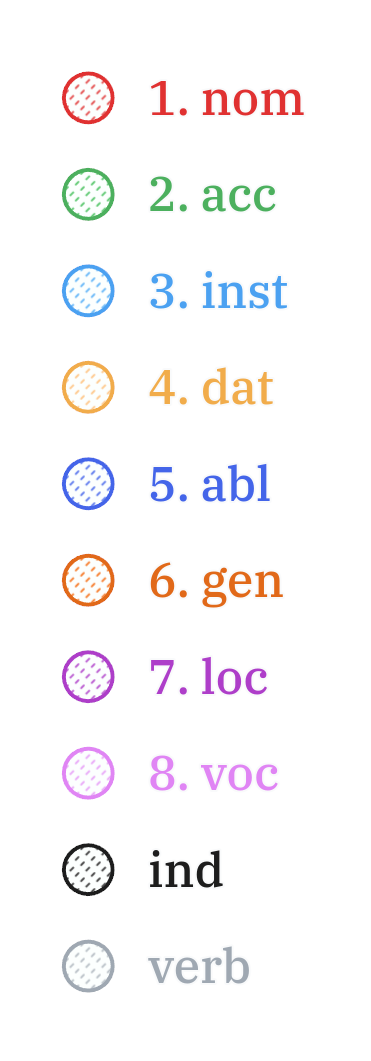
\includegraphics[width=25mm]{./images/cases-legend-white-large.png}%
    }%
  }%
}

\newcommand*\sentenceDiaMsg{\textbf{Exercise:} Draw a sentence analysis diagram below and indicate declensions.}

\newcommand*\sentenceDiaSolution[2][0.4]{%
  \ifanswerkey%
    \hspace*{-\spinemargin}%
    \begin{minipage}{\paperwidth}%
      \centering%
      \includegraphics[scale=#1]{#2}%
    \end{minipage}%
  \else%
    \settototalheight{\@tmp@height}{\includegraphics[scale=#1]{#2}}%
    \begin{minipage}[\@tmp@height]{\linewidth}%
      \sentenceDiaMsg%
    \end{minipage}%
  \fi%
}

\usepackage{cwpuzzle}

\renewcommand\PuzzleCluePre{%
  \begin{minipage}[t]{0.75\linewidth}%
}

\renewcommand\PuzzleClueFont{\fontsize{11}{17}\selectfont}

% \def\PuzzleThickline{\linethickness{2pt}}

\makeatother
\relax \yournamefalse
\date{\today}
\title{Pali Readings}
\hypersetup{
 pdfauthor={The Bhikkhu Saṅgha},
 pdftitle={Pali Readings},
 pdfkeywords={},
 pdfsubject={},
 pdfcreator={Emacs 30.0.50 (Org mode 9.6.6)}, 
 pdflang={En_Gb}}
\begin{document}

\maketitle
\frontmatter

{\centering

{\Huge Pāḷi Readings}

\bigskip
\href{https://vinaya-class.github.io}{https://vinaya-class.github.io}

{\scshape\small last updated on}\\
\today

}

\bigskip
\tableofcontents*

\mainmatter

\chapter{Ratana Sutta Paritta (Snp 2.1)}
\label{sec:org1f18b61}

\newlength{\colOne}\setlength{\colOne}{0.3\linewidth}
\newlength{\colTwo}\setlength{\colTwo}{0.65\linewidth}

\begin{spacedquote}
Yaṁ kiñci vittaṁ idha vā huraṁ vā, \\[0pt]
Saggesu vā yaṁ ratanaṁ paṇītaṁ; \\[0pt]
Na no samaṁ atthi tathāgatena, \\[0pt]
Idampi buddhe ratanaṁ paṇītaṁ; \\[0pt]
Etena saccena suvatthi hotu.
\end{spacedquote}

\begin{longtable}{L{\colOne} L{\colTwo}}
yaṁ kiñci (ind.) [yaṃ + kiṃ + ci] & whatever; everything; all\\[0pt]
vitta (nt.) & (1) wealth; property (2) delight; pleasure; lit. got\\[0pt]
huraṁ (ind.) & there; in another world\\[0pt]
sagga (m.) & heaven; paradise\\[0pt]
ratana (nt.) & (1) jewel; gem (2) treasure (3) queen\\[0pt]
paṇīta (adj.) & fine; superior; sublime; lit. brought forward\\[0pt]
sama (adj.) & (1) level; even; balanced (2) like; equal (to); same (as)\\[0pt]
sacca (nt.) & truth\\[0pt]
suvatthi (f.) [su + √as + ti] & well being; prosperity\\[0pt]
\end{longtable}

\begin{spacedquote}
Khayaṁ virāgaṁ amataṁ paṇītaṁ, \\[0pt]
Yadajjhagā sakyamunī samāhito; \\[0pt]
Na tena dhammena samatthi kiñci, \\[0pt]
Idampi dhamme ratanaṁ paṇītaṁ; \\[0pt]
Etena saccena suvatthi hotu.
\end{spacedquote}

\enlargethispage{\baselineskip}

\begin{longtable}{L{\colOne} L{\colTwo}}
khīyati & is destroyed; is exhausted\\[0pt]
khīṇa (pp. of khīyati) & consumed; destroyed\\[0pt]
khaya (m. from khīyati) & wearing away; destruction\\[0pt]
virāga (m.) & fading of desire (for); dispassion (towards)\\[0pt]
amata (nt.) & (1) deathless state; immortality (2) deathless; immortal; undying\\[0pt]
adhigacchati & gets to; attains; obtains; lit. arrives at\\[0pt]
ajjhagā (imperf. of adhigacchati) & got; obtained; achieved; lit. arrived at\\[0pt]
samādahati & (1) (of the mind) composes; stabilizes; collects (2) (of fire) kindles; lights; lit. puts together\\[0pt]
samāhita (pp. of samādahati) & composed; centred; settled\\[0pt]
\end{longtable}

\clearpage

\begin{spacedquote}
Yaṁ buddhaseṭṭho parivaṇṇayī suciṁ, \\[0pt]
Samādhimānantarikaññamāhu; \\[0pt]
[samādhiṃ + ānantarikaṃ + yaṃ + āhu] \\[0pt]
Samādhinā tena samo na vijjati, \\[0pt]
Idampi dhamme ratanaṁ paṇītaṁ; \\[0pt]
Etena saccena suvatthi hotu.
\end{spacedquote}

\begin{longtable}{L{\colOne} L{\colTwo}}
seṭṭha (adj.) & (1) foremost; supreme; (2) chief; leader\\[0pt]
vaṇṇayati & (1) praises; extols (2) comments on; interprets; explains\\[0pt]
parivaṇṇayati & describes; recommends; extolls; lit. praises all around\\[0pt]
suci (adj.) & (1) clean; pure (2) (of tastes and smells) good; fine\\[0pt]
antara (nt.) & space between; interval; distance\\[0pt]
ānantarika (adj.) & immediate; without delay; with immediate results\\[0pt]
ahu / ahosi (aor. of hoti) & was; existed; became\\[0pt]
vijjati [√vid + ya + ti] & (1) exists; is found; is present (2) is possible\\[0pt]
\end{longtable}

\begin{spacedquote}
Ye puggalā aṭṭha sataṁ pasatthā, \\[0pt]
Cattāri etāni yugāni honti; \\[0pt]
Te dakkhiṇeyyā sugatassa sāvakā, \\[0pt]
Etesu dinnāni mahapphalāni; \\[0pt]
Idampi saṅghe ratanaṁ paṇītaṁ, \\[0pt]
Etena saccena suvatthi hotu.
\end{spacedquote}

\begin{longtable}{L{\colOne} L{\colTwo}}
puggala (m.) & person; individual\\[0pt]
sarati & (1) remembers; recollects (2) drifts; wanders; flows\\[0pt]
sata (adj. pp. of sarati) & mindful; present; attentive\\[0pt]
pasaṃsati & praises; approves (of); commends\\[0pt]
pasattha (pp. of pasaṃsati) & praised; commended; exalted\\[0pt]
yuga (nt.) & (1) yoke (2) pair; set of two\\[0pt]
dadāti & gives (to); offers (to)\\[0pt]
dinna (pp. of dadāti) & given (to); offered (to)\\[0pt]
phala (nt.) & (1) fruit; berry (2) consequence; result\\[0pt]
\end{longtable}

\clearpage

\begin{spacedquote}
Ye suppayuttā manasā daḷhena, \\[0pt]
Nikkāmino gotamasāsanamhi; \\[0pt]
Te pattipattā amataṁ vigayha, \\[0pt]
Laddhā mudhā nibbutiṁ bhuñjamānā; \\[0pt]
Idampi saṅghe ratanaṁ paṇītaṁ, \\[0pt]
Etena saccena suvatthi hotu.
\end{spacedquote}

\begin{longtable}{L{\colOne} L{\colTwo}}
payuñjati & harnesses; employs; applies\\[0pt]
payutta (pp. of payuñjati) & intent; engaged\\[0pt]
suppayutta (adj.) [su + payutta] & fully engaged; diligently practising\\[0pt]
manasa (adj.) & focused on; lit. with such a mind\\[0pt]
daḷha (adj.) & strong; firm; steady\\[0pt]
nikkāmī (adj.) [nī + √kam + *ī] & striving (in); active (in); lit. going out\\[0pt]
pāpuṇāti & reaches; attains; arrives (at)\\[0pt]
patti (f. abstr. from pāpuṇāti) & (1) reaching; getting (2) profit; share; lit. what is obtained\\[0pt]
patta (pp. of pāpuṇāti) & reached; attained; have arrived (at)\\[0pt]
vigāhati & enters, plunges into\\[0pt]
vigayha (ger. of vigāhati) & plunging into; diving into\\[0pt]
labhati & gets; receives; obtains\\[0pt]
laddhā (abs. of labhati) & having got; having obtained\\[0pt]
mudhā (ind.) & for free; freely; gratis; for nothing\\[0pt]
nibbuti (f.) [nī + √vā + ti] & quenching; cooling; lit. blown away state\\[0pt]
bhuñjamāna (prp. of bhuñjati) & eating; consuming; enjoying\\[0pt]
\end{longtable}

\clearpage

\begin{spacedquote}
Khīṇaṁ purāṇaṁ nava natthi sambhavaṁ, \\[0pt]
Virattacittāyatike bhavasmiṁ; \\[0pt]
Te khīṇabījā avirūḷhichandā, \\[0pt]
Nibbanti dhīrā yathāyaṁ padīpo; \\[0pt]
Idampi saṅghe ratanaṁ paṇītaṁ, \\[0pt]
Etena saccena suvatthi hotu.
\end{spacedquote}

\begin{longtable}{L{\colOne} L{\colTwo}}
khīyati & is destroyed; is exhausted\\[0pt]
khīṇa (pp. of khīyati) & consumed; destroyed\\[0pt]
khaya (m. from khīyati) & wearing away; destruction\\[0pt]
purāṇa (adj.) & previous; old; ancient\\[0pt]
nava (adj.) & new; fresh\\[0pt]
sambhavati & comes to be; happens; occurs\\[0pt]
sambhava (m. from sambhavati) & birth; origin; source (of)\\[0pt]
rajjati & finds pleasure (in); is enamoured (with)\\[0pt]
virajjati & becomes detached (from); loses interest (in)\\[0pt]
viratta (pp. of virajjati) & detached (from); without desire (for); lost interest (in)\\[0pt]
āyati (f.) & future; upcoming\\[0pt]
āyatika (adj. from āyati) & upcoming; future\\[0pt]
bīja (nt.) & seed; germ\\[0pt]
virūḷhi (f.) & growth; increase\\[0pt]
chanda (m.) & (1) interest; desire; wish (2) consent; agreement\\[0pt]
dhīra (adj.) & (1) stable; constant; reliable; firm (2) wise; intelligent\\[0pt]
padīpa (m.) & lamp; light; lighting\\[0pt]
\end{longtable}
\end{document}